\documentclass{ieeeaccess}

% set font encoding for PDFLaTeX, XeLaTeX, or LuaTeX
\usepackage{ifxetex,ifluatex}

\if\ifxetex T\else\ifluatex T\else F\fi\fi T%
  \usepackage{fontspec}
\else
  \usepackage[T1]{fontenc}
  \usepackage[utf8]{inputenc}
  \usepackage{lmodern}
\fi

\usepackage{textcomp}
\usepackage{algorithmic}
%\usepackage{cite}
%\def\BibTeX{{\rm B\kern-.05em{\sc i\kern-.025em b}\kern-.08em
%    T\kern-.1667em\lower.7ex\hbox{E}\kern-.125emX}}
\usepackage{amsmath}
\usepackage{amssymb}
\usepackage{amsthm}
\usepackage{bm}
\usepackage{bbm}
\usepackage{mathtools}
\usepackage{physics}

\usepackage{enumitem}
\usepackage{multicol}
\usepackage{graphicx}
\usepackage[dvipsnames]{xcolor}

\usepackage{hyperref}
\hypersetup{colorlinks=true,}

\usepackage[parfill]{parskip}
\usepackage{lipsum}
\usepackage[export]{adjustbox}
\usepackage{listings}

\usepackage{xparse} 
\usepackage{subfig} 
\usepackage{xparse} 
\usepackage{float}

\usepackage[sorting=none]{biblatex} 

%%%%%This is an image table command, can likely be deleted
\newcommand{\subf}[2]{

%
{\small 
\begin{tabular}
  [t]{@{}c@{}} #1\ 
  \#2 
\end{tabular}
}

%
} 

\makeatletter
\renewcommand*\env@matrix[1][c]{\hskip -\arraycolsep
  \let\@ifnextchar\new@ifnextchar
  \array{*\c@MaxMatrixCols #1}}
\makeatother
%%%%%% Tensor Product
\NewDocumentCommand{\tens}{e{_^}}{ 
\mathbin{\mathop{\otimes}\displaylimits \IfValueT{#1}{_{#1}} \IfValueT{#2}{^{#2}} }}
%%%%%% Add \R Reals
\newcommand{\R}{\mathbb{R}} 
\newcommand{\N}{\mathbb{N}} 
\newcommand{\Z}{\mathbb{Z}} 
%%%%%% Missing citation warn
\newcommand{\CITEMISSING}{\colorbox{BurntOrange}{CITE ME}}
%%%%%% Add \theorem float
\newtheorem{theorem}{Theorem}
%%%%%% Add \definition float
\theoremstyle{definition} 
\newtheorem{definition}{Definition}[section]
%%%%%%%%%%%%%%%%%%%%%%%%%%%%%%%%%%%%%%%%%%%%%%%%%%%%%%%%%%%%%%%%%%%%%%%%%%%%%%%%%%%%%%%%%%%%%%%%%%%%%%%%%%%%%%%%%%%%%%%%%%
%%%%%Uncomment to add citation library 
\bibliography{lib} 
\begin{document}
\title{Bayesian Local Phylodynamics for Outbreak Detection}
\author{David Helekal, Xavier Didelot}
\begin{abstract}
In epidemiology, it is often desirable to reconstruct the history of a pathogen population and it's structure. The problem of reconstructing the history of a pathogen population can be approached using phylodynamics. Phylodynamics utilises genomic data to assemble phylogenies, which are then used to infer the population size history. This is possible by viewing a phylogeny as a realisation of a coalescent process, with appropriately rescaled time. This approximation can be justified by viewing the coalescent process as a Wright-Fisher model, run backwards in time with the time rate equal to the population size. Within this report we will first introduce the coalescent process for phylodynamic inference, review its inhomogeneous generalisation, and finally introduce the main result of this work, a new model for the purpose of performing local phylodynamic inference. We intend for this model to enable us to make different inferences about the population history for different subsets of the whole population, and to enable the detection of and modelling of clonal expansions.
\end{abstract}
\titlepgskip=-15pt

\maketitle

\section{Introduction}
\PARstart{C}{lonal} expansions are a process in which a subset of the total population of a given bacterial strain undergoes explosive population growth that can be traced back to a particular individual \cite{smith_how_1993}. The presence of clonal expansions in bacterial populations has been of long-standing scientific interest and is implicated in epidemic processes, were an outbreak can be traced to a single ancestor \cite{smith_how_1993,spratt_displaying_2004,fraser_neutral_2005,ledda_re-emergence_2017}. This often happens when a  strain or an individual obtains a variant of a particular gene that confers evolutionary advantage, for example antibiotic resistance \cite{holden_genomic_2013,hsu_evolutionary_2015, ledda_re-emergence_2017}.\\
The presence of clonal expansions leaves an imprint in the overall population structure of a given bacterial strain, with the topology of the phylogenetic tree associated with this often being referred to as star-like \cite{smith_how_1993,spratt_displaying_2004}.
Detecting hidden population structure corresponding to clonal expansions is a problem of interest in epidemiology and outbreak surveillance \cite{volz_identification_nodate}.\\
While methods for detecting inhomogeneities in the population structure and size have been studied since early days of genetic sequencing \cite{smith_how_1993,spratt_displaying_2004}, interest increased with whole genome sequencing becoming more accessible and affordable \cite{holden_genomic_2013,dearlove_measuring_2015,eldholm_four_2015}.\\
Despite the problems of inferring population size from a genealogy and detecting heterogeneities in the population structure being intrinsically tied, all but a couple of methods \cite{volz_identification_nodate,barido-sottani_multitype_2020}, to our knowledge, rely either on manual detection or indirect detection. We aim to develop a model for the formation of clonal expansions in genealogies using a structured coalescent process, and devise a bayesian method for joint estimation and detection of relative population sizes and clonal expansions.
\section{Existing Work}
\subsection{Phylodynamic Methods}
A phylogeny is a labeled tree, where leaf nodes correspond to sampling events, and internal nodes to the divergence of two separate clades from a common ancestor. Branch length labels correspond to time. As such a phylogeny can be viewed as a realisation of Kingman's Coalescent process. 
Kingman's Coalescent is a continuous time Markov chain (CTMC) stochastic process, defined on the state space ${1,2,3, ... ,K}$ which can be interpreted as a set of $j$ particles, where each pair of particles independently coalesces at a constant rate \cite{kingman_coalescent_1982}. This gives the transition rates:
\begin{gather}
g(j, j-1) = \binom{j}{2}\lambda\quad\lambda\in\R^+
\end{gather}
By taking a backwards in time approximation of the Wright-Fisher model, the coalescent process can be modified to model evolution of genealogies, i.e. how ancestors of a set of individuals relate to each other backwards in time. Denote the relative population size at time $t$ by $\alpha(t)$. Under such modification the transition rates become:
\begin{gather}
g(j, j-1) = \binom{j}{2}\cdot\frac{1}{\alpha(t)}
\end{gather}
\cite{griffiths_sampling_1994}\\
One way to interpret this is as a rescaling of time inversely proportional to the population size under Wright-Fisher model \cite{hein_gene_2004}.\\
As the transition rates depend on the relative population size, it is possible to utilise this model for the inverse problem of determining the history of the size of a population, based on genealogies reconstructed from genomic samples.
Such methods are often referred to as SkyLine methods first introduced in \cite{pybus_integrated_2000} and \cite{drummond_estimating_2002}.\\
The framework was then extended to allow for piecewise continuous population size functions \cite{gill_improving_2013} and to include covariates \cite{gill_understanding_2016}.
\subsection{Local Phylodynamics}
Whereas phylodynamics considers the size history of an entire population, the idea behind local phylodynamics is to consider the histories of selected subsets of related individuals, where each subset can be traced to a single ancestor. This can for example be practical when trying to detect hidden outbreaks, or clonal expansions due to a particular strain of a bacterium gaining a fitness advantage. This idea has been investigated in \cite{volz_identification_nodate}, where a null hypothesis based testing framework is developed to identify subsets of individuals that seem to have a significantly different population history than the the rest of the phylogeny. Recently, a birth-death type model that allows for heterogeneous growth rate parameters has been introduced in \cite{barido-sottani_multitype_2020}.
\section{Methods}
\subsection{Coalescent Preliminaries}
The coalescent process can be characterised as a time-inhomogeneous pure-death Markov process. We now conduct a brief analysis of the process and re-derive some properties.\\
The waiting times can be derived as follows:
For an inhomogenous CTMC, let $E_j(t)$ be the total exit rate from state $j$ at time $t$.
By the markov property individual exit events from a given state only depend on the state and given time, i.e. they form a time-inhomogeneous poisson process.
As such the probability of no events in an interval $[t,t+s],\quad s\in \R^+$ is 
\begin{gather}
\begin{aligned}
&\exp(-\int_t^{t+s}E_j(\tau)d\tau) =\\
&\exp(-\int_0^{s}E_j(t+\tau)d\tau)
\end{aligned}
\end{gather}
The waiting times are defined as:
\begin{gather}
W_j(t) = \inf\{s:X(t+s)\neq j \mid X(t) = j\}
\end{gather}
As such:
\begin{gather}
W_j(t) > s \Rightarrow \forall \tau\in[t, t+s]\quad X(\tau) = j
\end{gather}
Furthermore the above relation holds iff no exit event have occurred in the time interval $[t,t+s]$. As such:
\begin{gather}
\begin{aligned}
&P[W_j(t) > s] &=& P[\text{no exit events in }[t,t+s]]\\ 
&&=& \exp(-\int_0^{s}E_j(t+\tau)d\tau)
\end{aligned}
\end{gather}
And as such:
\begin{gather}
P[W_j(t) < s] = 1 - \exp(-\int_0^{s}E_j(t+\tau)d\tau)
\end{gather}
In the case of phylodynamic coalescent this becomes
\begin{gather}\label{eq:w_t}
P[W_j(t) \leq s] = 1 - \exp(-\int_0^{s}\frac{\binom{j}{2}}{\alpha(t+\tau)}d\tau)
\end{gather}
From equation \ref{eq:w_t} we can see that the waiting times between individual coalescent events depend on the relative population size.
\subsection{Simulating Phylogenies}
We are interested in simulating the scenario where sampling events and the relative population size is given. Denote the collection of sampling events in decreasing time order by:
\begin{gather}
\{s_j\}_{1\leq j\leq K}, \quad i>l \Leftrightarrow s_i \leq s_l\quad \forall i,l
\end{gather}
Under this scenario, phylogenies can be simulated as realisations of the inhomogenous coalescent process, conditioned on sampling events, using modified Gillespie's Algorithm \cite{erban_practical_nodate}. The key difference between standard Gillespie's Algorithm setting and our problem setting is that we need to condition on the sampling events.\\
Hence at any time greater than the earliest sampling event $t_i > s_K$ in the simulation, we first need to determine whether an event happens or not in the interval $[s_j, t_i]$ with $s_j = max\left\{s\in S : s<t_i\right\}$. Define $\Delta t_i \triangleq t_i-s_j$, and assume there are $j$ individual clades extant at time $t$. We are interested in the probability
\begin{gather*}
  P[W_j(t_i) > \Delta t_i] = \exp(-\int_0^{\Delta t_i}\frac{\binom{j}{2}}{\alpha(t+\tau)}d\tau)
\end{gather*}
To determine the next in simulation draw $r \sim \texttt{U}([0,1])$. 
If $r < P[W_j(t_i) > \Delta t_i]$, no events happen in the interval $[s_j, t_i]$. As such set $t_{i+1} = s_j$ and repeat the process.\\
If $r > P[W_j(t_i) > \Delta t_i]$ a coalescent event must happen in the interval $[s_j, t_i]$. Therefore we need to determine the next waiting time $W_j(t_i)$. The cumulative distribution function (CDF) of $W_j(t_i)$ is given by
\begin{gather}
\begin{aligned}
  P[W_j(t_i) < c \mid W_j(t_i) < \Delta t_i]\\
  = \frac{1-\exp(-\int_{0}^{c}{\frac{\binom{j}{2}}{\alpha(t+\tau)}d\tau})}{1-P[W_j(t_i) > \Delta t_i]}
\end{aligned}
\end{gather}
$W_j(t_i)$ can be generated by the inverse transform of exponentially distributed variables.\\ Let $W \sim \texttt{exp}(1)$ and note that random variates $W'$ with the CDF
\begin{gather}
  P[W' \leq c] = P[W\leq c\mid W\leq\Delta' t] \quad\forall c \leq \Delta t
\end{gather}
can be generated from random variables $u \sim \texttt{U}([0,1])$ by the following inverse transform
\begin{gather}
T(u) = -1\log[1-u(1-\exp(-\Delta' t))]
\end{gather} 
This can be justified as follows
\begin{gather*}
  P[T(u)\leq c] = P[u\leq T^{-1}(c)]
\end{gather*}
Using the property that $P[u\leq a] = a$ and requiring that $T(u)$ follows the same distribution as $W'$ we obtain
\begin{align*}
  &\Rightarrow& P[u\leq T^{-1}(c)] &= \frac{\int_0^c\exp(- t)dt}{\int_0^{\Delta t}\exp(- t)dt}\\
  &\Rightarrow& T^{-1}(c) &= \frac{1-\exp(- c)}{1-\exp(- \Delta t)}
\end{align*}
Being abled to generate appropriate random variates $W'$, a further inverse transform is applied, this time to obtain $W_j(t)$ from $W'$. First, we require that $\Delta' t$ be such that $P[W < \Delta' t]$ is equal to $P[W_j(t_i) < \Delta t]$. Next, we seek a function $G(W';t)$ such that
\begin{gather}
\begin{aligned}
&&P[W' \leq G^{-1}(c;t)] &= P[W_j(t) \leq c \mid W_j(t)\leq\Delta t]\\
&\Rightarrow& \frac{1-\exp(-G^{-1}(c;t))}{1-P[W > \Delta't]} &= \frac{1-\exp(-\int_{0}^{c}{\frac{\binom{j}{2}}{\alpha(t+\tau)}d\tau})}{1-P[W_j(t_i) > \Delta t_i]}
\end{aligned}
\end{gather}
Using that $1-P[W > \Delta't] = 1-P[W_j(t_i) > \Delta t_i]$ we obtain
\begin{gather}
\begin{aligned}
&\Rightarrow& &1-\exp(-G^{-1}(c;t))\\
&&=&  1-\exp(-\int_{0}^{c}{\frac{\binom{j}{2}}{\alpha(t+\tau)}d\tau})
\end{aligned}
\end{gather}
Where the inverse transform $G^{-1}$ is given by
\begin{gather}
\Rightarrow G^{-1}(c;t) = \int_{0}^{c}{\frac{\binom{j}{2}}{\alpha(t+\tau)}d\tau}\label{eq:inv_int}
\end{gather}\\
Therefore the scheme to generate waiting times $W_j(t)$ is to first generate appropriate $W'$ from uniformly distributed random variates, and then to further transform $W'$ by solving \ref{eq:inv_int}.\\
In practice, \ref{eq:inv_int} often cannot be solved analytically, and hence we resort to numeric methods.
\subsection{Inference Under Inhomogenous Coalescent}
The derivation of the likelihood function for time-inhomogenous coalescent process can be found in \cite{drummond_estimating_2002}. We adapt notational convention from \cite{drummond_estimating_2002}.
Let $\left\{t_i\right\}_{i\in S\subset \N}$ denote the times of events in increasing order. Let $t_Y\triangleq \left\{t_i\right\}_{i\in Y}$ denote times of coalescent events and $t_I\triangleq \left\{t_i\right\}_{i\in I}$ denote times of sampling events, where $Y$, $I$ are disjoint partitions of the index set $S$ with the property that $S = Y\cup I$.
The likelihood of a particular genealogy is then given by:
\begin{gather}
\begin{aligned}
\mathcal{L}\left(g\mid \alpha\right) 
= &\prod_{i\in S\setminus 1}&\left(\mathbbm{1}_Y(i)\frac{\binom{k_{i}}{2}}{\alpha(t_i)}+\mathbbm{1}_I(i)\right)\\
&&\cross\exp(-\int_{t_{i-1}}^{t_i}\frac{\binom{k_{i}}{2}}{\alpha(\tau)}d\tau)
\end{aligned}
\end{gather}
The log-likelihood is:
\begin{gather}
\log\mathcal{L}\left(g\mid \alpha\right) 
= -\sum_{i\in S\setminus 1}{\int_{t_{i-1}}^{t_i}{\frac{\binom{k_{i}}{2}}{\alpha(\tau)d\tau}}} + \sum_{i\in Y}{\log\frac{\binom{k_{i}}{2}}{\alpha(t_i)}}
\end{gather}
\subsection{Coalescent with Local Population Structure}
We now present novel local phylodynamic model.
In order to help illustrate the concepts behind this model, consider the following scenario.:
Suppose we sequence the genomes of a set of pathogenic bacterial samples. 
At an unknown point in time a particular strain acquired a mutation which conferred resistance to a widely used antibiotic. This increases the strain's fitness and enables it to undergo a period of rapid growth leading to a clonal expansion. Assuming that this increase in fitness occurs in a short time span, the clade -- a set of lineages sharing the same common ancestor, of this strain will behave differently in the phylogenetic tree. The clade corresponding to this strain will have a coalescent rate corresponding to a rapidly expanding population starting from a very small number of individuals.\\
The problem of identifying hidden population structure has been proposed in \cite{volz_identification_nodate}, where a testing based approach was used to identify structure in a phylogeny, as well as in \cite{barido-sottani_multitype_2020}, where a birth-death type model was used.\\
In our approach, we will build upon the standard coalescent model, modifying it as to allow for change points located on the branches of the phylogeny, marking the event when a particular clade starts behaving according to a different population size function than its parent clade.\\
In our model, coalescent nodes have an added colour property, and each colour coalesces according to a colour specific, time dependent case. Nodes of non-identical colour can coalesce iff at least one of them is the last remaining node of a given colour.
Different colours correspond to different clades, each behaving under its own growth function.\\
Similar models have been used in epidemiology to track outbreaks \cite{maio_scotti_2016}, or transmission chains \cite{didelot_genomic_2017}.
These models are often called structured coalescent process, effectively adding a colour property to the vertices of phylogenies.
%%%%%%%%%%%%%%%%%%%%%%%%%%%%%%%%%%%%%%%%%%%%%%%%%%%%%%%%%%%%
%%%%%%%%%%%%%%%%%%%%%%%%%%%%%%%%%%%%%%%%%%%%%%%%%%%%%%%%%%%%
%%%%%%%%%%%%%%%%%%%%%%%%%%%%%%%%%%%%%%%%%%%%%%%%%%%%%%%%%%%%
%%%%%%%%%%%%%%%%%%%%%%%%%%%%%%%%%%%%%%%%%%%%%%%%%%%%%%%%%%%%
\subsubsection{Model}
A given genealogy $\mathbf{g}=(V_\mathbf{g}, E_\mathbf{g}, t_\mathbf{g})$ is an incomplete, empirical sample of the underlying process.\\
It consists of nodes $V_\mathbf{g}$, directed edges $E_\mathbf{g}$, and node labels $t_\mathbf{g}$ corresponding to event times.\\
The genealogy $\mathbf{g}$ shall be indexed by an index set $S=1\leq i \leq N\subset \N$, with $Y\subset S$ corresponding to coalescent events and $I\subset S$ corresponding to sampling events.\\
For convenience, assume that all edges are in the forwards time direction, i.e.: 
\begin{gather*}
\forall k,l \in S: (k,l)\in E_\mathbf{g} \Rightarrow t_k<t_l
\end{gather*}
Furthermore, all event times are ordered in descending (backwards) time order, with the first event corresponding the the most recent sample
\begin{gather*}
\forall k,l \in S: k<l \Rightarrow t_k > t_l
\end{gather*}
Under the assumption that $\mathbf{g}$ is a genealogy of a given sample, with each edge in $E_\mathbf{g}$ there is an associated unobserved set of individuals descending from one another. At some point along an edge from one lineage to another, the lineage can undergo a colour change, and become the most recent ancestor of a diverging clade. This event corresponds to this lineage somehow gaining advantage over other lineages, be it a bacterium gaining resistance against a drug, or a strain of a virus invading a completely susceptible population.
\begin{definition}[Multiple Lineage Coalescent]\label{def:model}
Given $M$ colours, $M$ population size functions $\mathbf{\alpha}\triangleq\{\alpha_j(t)\}_{1\leq j\leq M}$. Let $Y(t)$ be a CTMC with the state space:
\begin{gather}
  \Sigma = \left\{\mathbf{s}\in \Z_+: |\mathbf{s}|\geq1\right\}
\end{gather}
and the transition rates
\begin{gather}\label{eq:multirate}
\begin{align}
\mathbf{s}&\to\mathbf{s}-\mathbf{e_j} &\quad& \binom{s_j}{2}\alpha_j^{-1}(t)&\quad&1\leq j\leq M\\
\mathbf{s}&\to\mathbf{s}-\mathbf{e_j}+\mathbf{e_k}&\quad& \delta_{1,j}\beta s_k&\quad&1\leq j,k\leq M
\end{align}
\end{gather}
Where $\beta$ is an unknown rate.
\end{definition}
The interpretation of this model in backwards (coalescent) time is that each node corresponds to a single specific clade (colour). Nodes of the same clade coalesce at i.i.d rates, according to a clade specific growth functions, until reaching the most recent common ancestor (MRCA) of given clade. The MRCA then changes type (colour) to that of a different clade. \\
Under the hypothesis, along each of the edges from the parent of a clade MRCA to the MRCA lies a point in that characterises the time of divergence of the clade, after which the clade starts to undergo clonal expansion.
\subsubsection{Inference}
Assume that we have been given a genealogy as described in previous section. The number of individual clades $M$, the effective population size functions $\mathbf{\alpha}$, and the placement and divergence events in descending order $\Xi =\{\xi_i\}_{1\leq i\leq M}$, are unknown. In effect we seek to infer the posterior using the following factorisation:
\begin{gather}
\mathcal{L}(\mathbf{\alpha}, \Xi, M\mid\mathbf{g}) \propto 
\mathcal{L}(\mathbf{g}\mid \Xi, M, \mathbf{\alpha})\mathcal{L}(\mathbf{\alpha}\mid\Xi,M)\mathcal{L}(\Xi,M)
\end{gather}\\
\begin{gather}
\mathcal{L}(\mathbf{g}\mid \Xi, M, \mathbf{\alpha})
\end{gather}
\begin{definition}[Divergence Event] A divergence event $\xi$ associated with a clade is a tuple:
\begin{gather}
\xi=\left(e', \tau\right)
\end{gather}
where $\tau$ denotes the time of the divergence event, and $e' = (v^{pa}, v^{MRCA}) \in E_{\mathbf{g}}$ denotes the edge along which the divergence event happens, with $v^{MRCA}$ being the MRCA of the newly diverging clade.
\end{definition}
In order to identify the likelihood $\mathcal{L}(\mathbf{g}\mid \Xi, M, \mathbf{\alpha})$, the genealogy needs to be first partitioned into separate subtrees, each corresponding to an individual clade.
\begin{definition}[Descendant Set]
\begin{gather}
\begin{aligned}
\mathcal{D}(i) &\triangleq \{j\in S\mid j \text{ is a descendant of } i\}
\end{aligned}
\end{gather} 
\end{definition}
As lineages within a clade can only coalesce with one another, the coalescence rate is independent of other clades, and the time of divergence has been given, the total likelihood can be derived as the product of individual clade specific likelihoods.
\begin{definition}[Lineage Subtree]
A subtree $W(\xi_i)$ associated with a divergence event $\xi_i$ consists of all vertices, edges and times associated with a given clade.
\begin{gather}
W(\xi_i) \triangleq \mathcal{D}(v^{pa}_i) \setminus \bigcup_{j<i}(\mathcal{D}(v^{pa}_j))
\end{gather} 
\end{definition}
A final step before deriving clade specific likelihoods is required, that is, the divergence times have to be included along with the times contained within the clade subtree. These behave identically to sampling events.\\

Denote the set of all divergence times associated with a Lineage Subtree $W(\xi_j)$ $\tau_{W(\xi_j)}$
\begin{gather*}
\tau_{W(\xi_j)} \triangleq \tau_i \in \xi_i : v^{pa}_i \in W(\xi_j), \quad \forall 1\leq i\leq M
\end{gather*}
Finally define the set of all times associated with a particular clade
$T(\xi_j) = \tau_{W(\xi_j)}\cup t_{W(\xi_j)}$, indexed by set $S_{T(\xi_j)}=\{1 ... |T(\xi_j)|\}$ such that
\begin{gather*}
\forall t_k, t_l \in T(\xi_j),\quad k>l \Rightarrow t_k \geq t_l
\end{gather*}
Let $k_{i,\xi_j}$ denote the number of extant individuals corresponding to clade subtree  $\xi_j$ during the time interval $[t_{i-1}, t_i]$.
The total likelihood is equal to:
\begin{gather}
\mathcal{L}(\mathbf{g}\mid \Xi, M, \mathbf{\alpha}) = \prod_{j=1}^{M}\mathcal{L}(T(\xi_j) \mid \alpha_j) 
\end{gather}
\begin{gather}
\begin{aligned}
\mathcal{L}(T(\xi_j) \mid \alpha_j) = \prod_{t_i\in T(\xi_j)}&\left(\mathbbm{1}_{t_Y}(t_i) \frac{\binom{k_{i,\xi_j}}{2}}{\alpha_j(t_i)}+\mathbbm{1}_{t_I\cup\tau_{W(\xi_j)}}(t_i)\right)\\
&\cross\exp(-\int_{t_{i-1}}^{t_i}\frac{\binom{k_{i,j}}{2}}{\alpha_j(\tau)}d\tau)
\end{aligned}
\end{gather}
\subsubsection{Choice of Population Size Functions} 
While the parent clade is assumed to be at equilibrium, the population size functions of the diverging clades have to satisfy several properties.\\
First we introduce the variable $\tau = -t + T_{max} - T_{div}$ which denotes time relative to a divergence event of a given clade, where $T_{div}$ denotes the divergence time and $T_{max}$ denotes the time of the most recent sample.
In our model we assume that the diverging subpopulation only appears after the divergence event, and as such it is required that at time $\tau=0$ the population vanishes $\alpha(\tau)=0$. Furthermore, we are looking for a monotone decreasing function in $\tau$, that exhibits saturating behaviour as $\tau$ grows large.
Initially, functions exhibiting a period of exponential growth were investigated, however these were ill-posed numerically.
Hence we arrived at the following function
\begin{gather}
\alpha(\tau) = K\frac{r\tau^2}{1+r\tau^2}
\end{gather} 
Where $K$ is the carrying capacity and $r$ is the growth rate.
This function  exhibits saturating behaviour, symmetry around zero, and numerically stable behaviour due to both not relying on time-offsetting exponentials, and separately also having a more gradual decay around zero.\\
\begin{figure}[H]
  \centering
     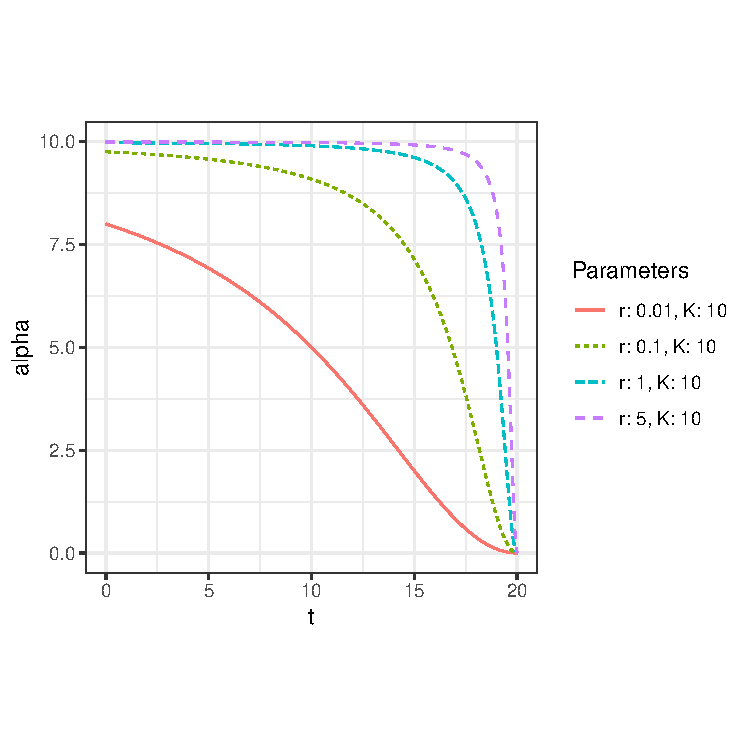
\includegraphics[width=0.4\textwidth]{../R/alpha_plots}
    \caption{$\alpha(\tau)$ under different parameters, with $T_{div}=20$}
\end{figure}
The integral of the reciprocal $\alpha^{-1}(\tau)$ under this formulation is then given by 
\begin{gather}
\begin{aligned}\label{eq:rint}
&\int_{t}^{t+s}\alpha^{-1}(\tau)\,d\tau\\ &= \frac{1}{K}\left[-\frac{1}{r(\tau-T_{max}+T_{div})}+\tau-T_{max}+T_{div}\right]_{t}^{t+s}
\end{aligned}
\end{gather}
As $t+s$ approaches the divergence time relative to the most recent sample $T_{div} - T_{max}$, the rate integral \ref{eq:rint} approaches infinity, and as such all coalescence within a clade happens before time of divergence with probability one.
\section{Results}
\subsection{Implementation Notes}
The framework described is being implemented as an R package, featuring the ability to simulate genealogies under the model we propose, compute model likelihoods for varying parameters. and to perform inference under same model using MCMC. Please note, as this is unpublished and work in progress, the repository is currently private; access will be granted upon request. Once this has been submitted for publication and completed, the package will be released under an open source license.
\subsection{Exponential Growth}
\subsubsection{MCMC Inference}
First thing that has been implemented and tested was a basic framework that enables simulating genealogies under the standard inhomogenous coalescent process, and the computation of likelihoods under the standard inhomogenous coalescent model. Along with this, standard Metropolis-Hastings MCMC routine was implemented and subsequently tested by simulating a genealogy undergoing exponential growth, and performing inferences on the rate parameter and the maximum population size parameter, effectively replicating results in \cite{drummond_estimating_2002}.\\
This example used the relative population size function $\alpha(t) = N*\exp(-\lambda t)$, and consisted of 100 sampling events between 0 and 10 years before present.
Accordingly, a genealogy has then been simulated with a rate parameter $\lambda$ and final size parameter $N$ drawn from a uniform densities on intervals $[0.1, 10]$, and $[1,100]$ respectively.\\
A Metropolis-Hastings MCMC scheme was then used to infer the parameters $\lambda$ and $N$. An exponential distribution rate equal to one was chosen as the prior for $\lambda$, as well as for $N$.\\
One million iterations were used and the first one hundred thousand were discarded as burn in time. To further validate the fit, both a maximum likelihood (MLE) and maximum \textit{a-posteriori} (MAP) estimates were computed and plotted against the posterior marginals inferred by the MCMC \ref{hists:a, hists:b}.
%%%%%%%%%%%%%%%%%%%%%%%%%%%%%%%%%%%%%%%%%%%%%%%%%%%%%%%%%%%%
%%%%%%%%%%%%%%%%%%%%%%%%%%%%%%%%%%%%%%%%%%%%%%%%%%%%%%%%%%%%
%%%%%%%%%%%%%%%%%%%%%%%%%%%%%%%%%%%%%%%%%%%%%%%%%%%%%%%%%%%%
%%%%%%%%%%%%%%%%%%%%%%%%%%%%%%%%%%%%%%%%%%%%%%%%%%%%%%%%%%%%
\begin{figure}[H]
  \centering
  \subfloat[]{\label{trace:a}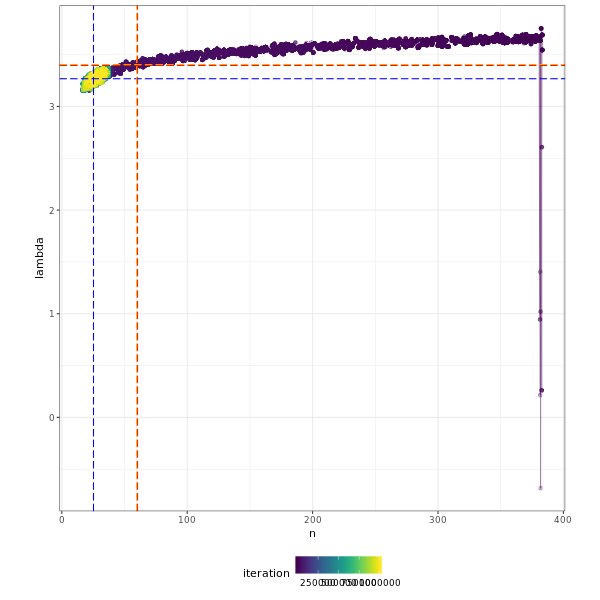
\includegraphics[scale=.25]{../R/trace}}

  \subfloat[]{\label{trace:b}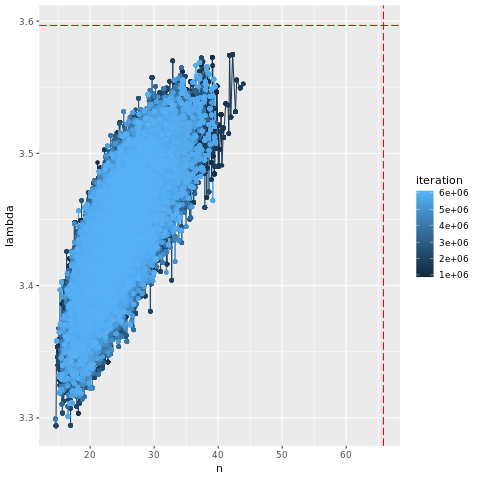
\includegraphics[scale=.25]{../R/trace_zoom}}
  \caption{Trace plots for the Markov chain. Red lines denote true parameter values. MLE marked by orange lines. MAP marked by blue lines. \ref{trace:a} Shows the entire trace of the chain. \ref{trace:b} Shows the trace with the first 100000 iterations discarded. Colour gradient corresponds to the iteration number, with more recent iterations in yellow.}
  \label{fig:trace}
\end{figure}
%%%%%%%%%%%%%%%%%%%%%%%%%%%%%%%%%%%%%%%%%%%%%%%%%%%%%%%%%%%%
%%%%%%%%%%%%%%%%%%%%%%%%%%%%%%%%%%%%%%%%%%%%%%%%%%%%%%%%%%%%
%%%%%%%%%%%%%%%%%%%%%%%%%%%%%%%%%%%%%%%%%%%%%%%%%%%%%%%%%%%%
%%%%%%%%%%%%%%%%%%%%%%%%%%%%%%%%%%%%%%%%%%%%%%%%%%%%%%%%%%%%
\begin{figure}[H]
  \centering
  \subfloat[]{\label{hists:a}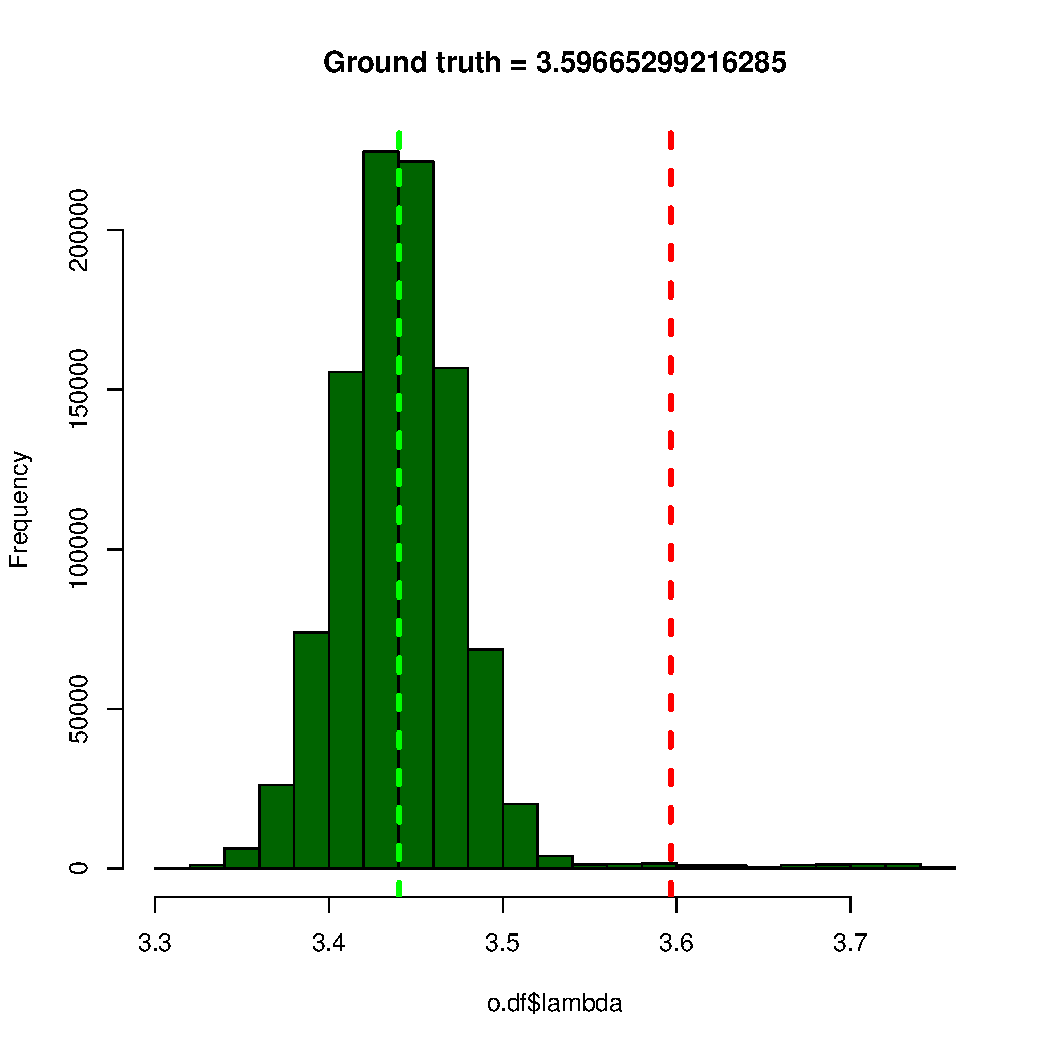
\includegraphics[scale=.4]{../R/lambdahist}}
  
  \subfloat[]{\label{hists:b}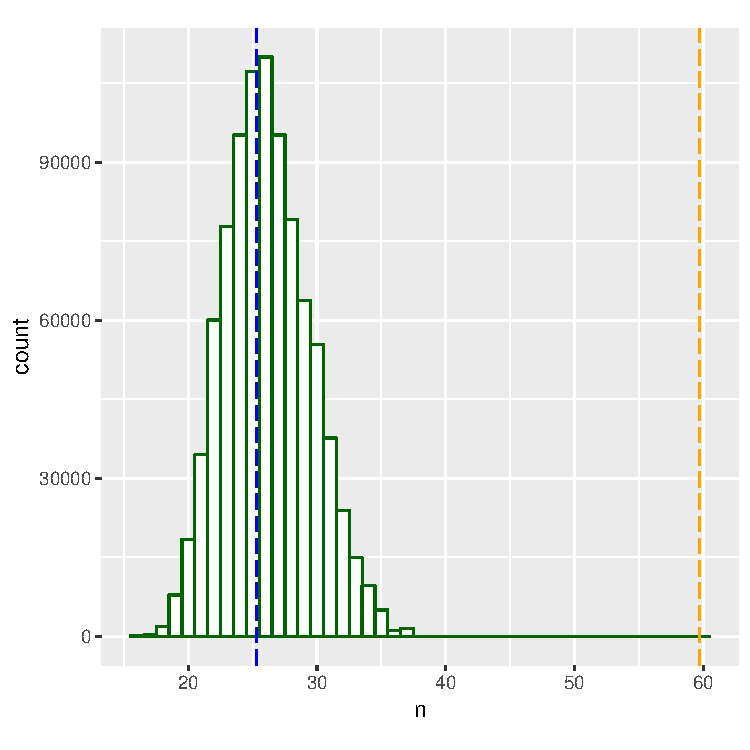
\includegraphics[scale=.4]{../R/nhist}}
  \caption{Histograms of the posterior marginals. MLE marked by orange line. MAP marked by blue line. \ref{hists:a} $\lambda$ marginal \ref{hists:b} $N$ marginal}
  \label{fig:hists}
\end{figure}
\begin{figure}[H]
  \centering
    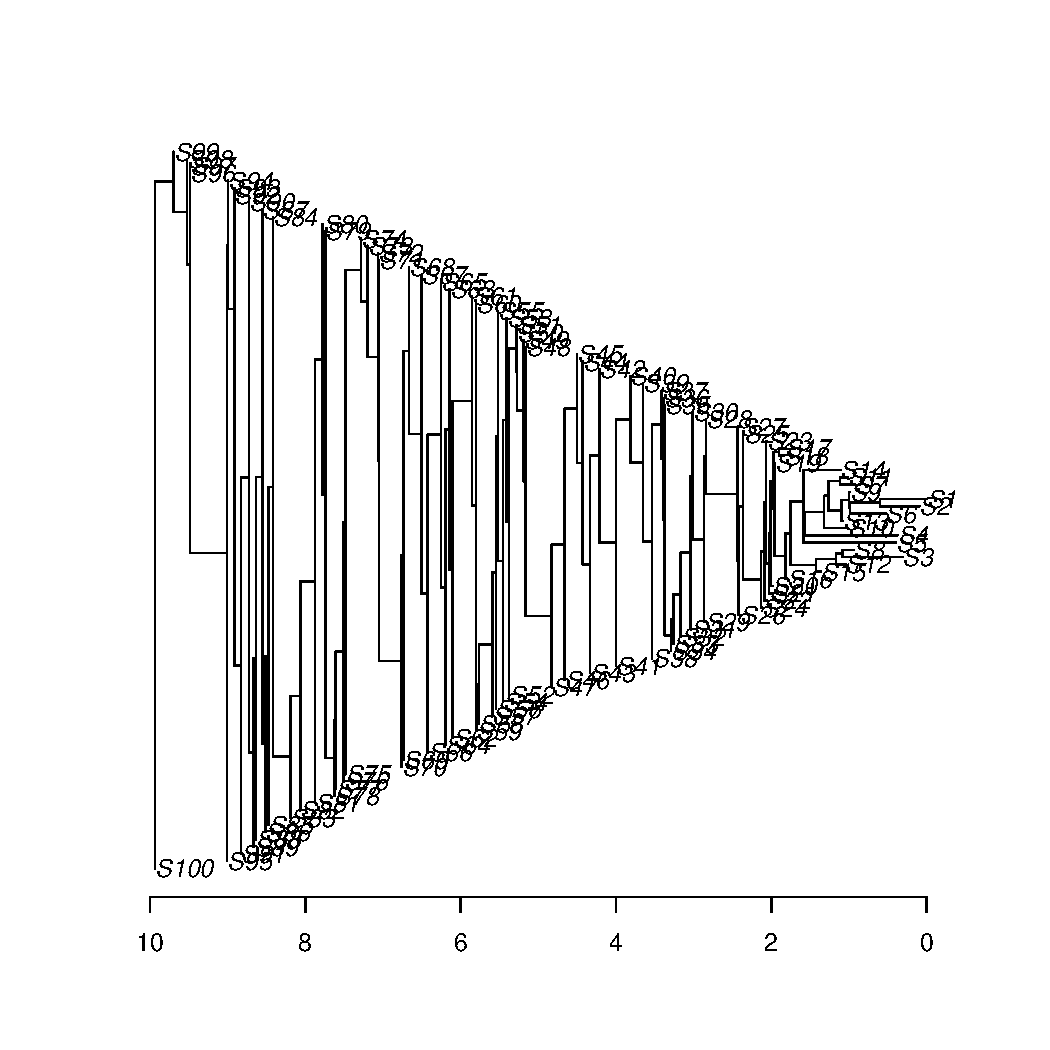
\includegraphics[width=0.4\textwidth]{../R/tree}
    \caption{The simulated genealogy used for this example.}
\end{figure}'
%%%%%%%%%%%%%%%%%%%%%%%%%%%%%%%%%%%%%%%%%%%%%%%%%%%%%%%%%%%%
%%%%%%%%%%%%%%%%%%%%%%%%%%%%%%%%%%%%%%%%%%%%%%%%%%%%%%%%%%%%
%%%%%%%%%%%%%%%%%%%%%%%%%%%%%%%%%%%%%%%%%%%%%%%%%%%%%%%%%%%%
%%%%%%%%%%%%%%%%%%%%%%%%%%%%%%%%%%%%%%%%%%%%%%%%%%%%%%%%%%%%
\subsection{Coalescent with Local Population Structure}
\subsubsection{Phylogeny Simulation}
The package in development is currently capable of simulating phylogenies based on the coalescent process with local population structure proposed in this work. 
Phylogenies can be simulated with an arbitrary number of diverging subpopulations and clearly visualised.\\
The package is also capable of rapidly computing likelihoods for the arbitrary phylogenies and parameters. The likelihood computation is partly implemented in C++ for increased performance. 
\begin{figure}[H]
  \centering
     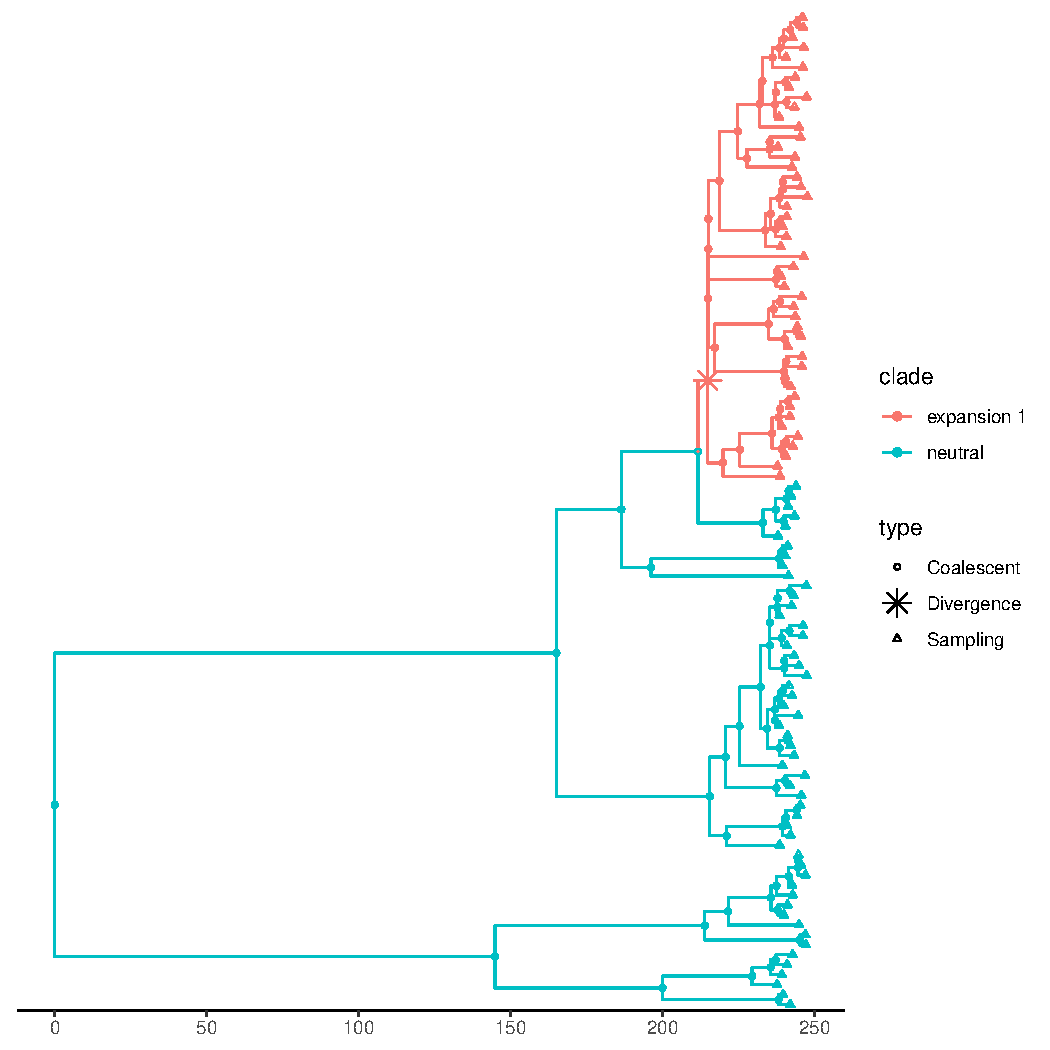
\includegraphics[width=0.5\textwidth]{../R/tree_structured}
    \caption{A simulated genealogy with one clonal expansion}
\end{figure}
\begin{figure}[H]
  \centering
     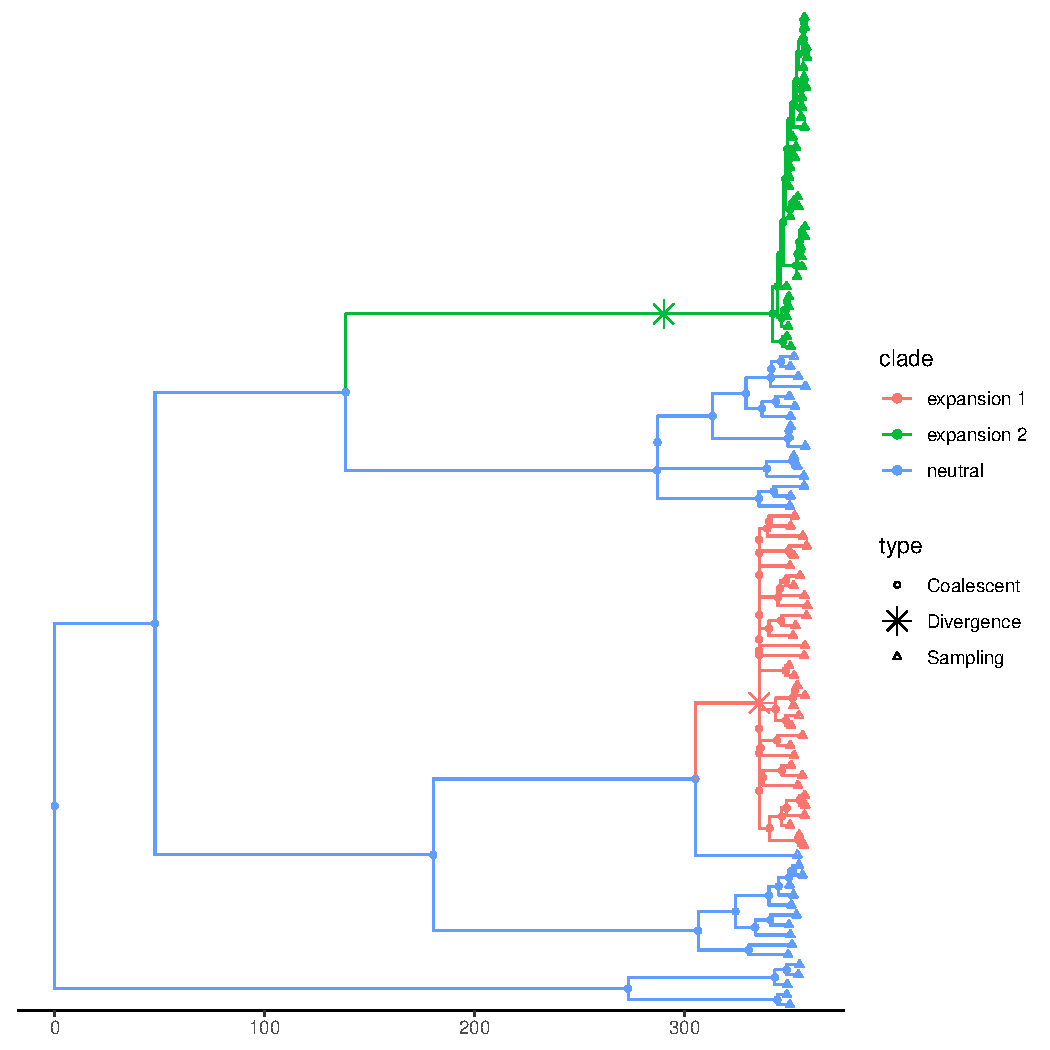
\includegraphics[width=0.5\textwidth]{../R/2events/tree_structured}
    \caption{A simulated genealogy with four clonal expansions}
\end{figure}
\subsubsection{MCMC inference}
At the moment we are in the process of implementing, and validating the MCMC routine for inference under coalescent with local population structure, and with a fixed number of divergence events. Currently there is a bug in the proposal move of the MCMC algorithm that changes the location of the divergence event, specifically, when it's supposed to traverse the root of the tree. As such we are unable to present reliable results at the moment. 
\section{Discussion \& Future Work}
\section{Discussion}
In this work we proposed a framework to enable local phylodynamic inference, with the aim to facilitate usage of genomic data for outbreak detection.
We implemented this model in an R package which we plan to release as open source on github once completed. To our knowledge this is a novel model, and there are no other models designed to capture the process of clonal expansions in genealogies.\\
At the moment we are still debugging implementation issues with the MCMC routine for the coalescent with local population structure, and these need to be addressed before thoroughly testing the MCMC inference on simulated data.\\ 
The effect of priors and of the choice of the population size function family for divergence events has not been properly investigated. It would be desirable to investigate what effect do different function families and parameter priors have on inference under our model.\\
Furthermore, it would be worth investigating the analytic properties of proposed model, and to see whether it can be shown to be consistent with existing models in population genetics in the limit, under appropriate assumptions.\\ 
\section{Future Work}
Once work on the MCMC routine for a fixed number of divergence events is completed and the routine is validated, we will move onwards to expand this to an arbitrary number of divergence events.\\
Having a variable amount of divergence events leads to the dimensionality of the problem not being fixed, and therefore will require the use of Reversible Jump MCMC (RjMCMC) \cite{green_reversible_1995, fan_reversible_2010}, which is computationally intensive.\\
If the performance of this framework in this setting is satisfactory, a further comparison with existing methods such as \cite{volz_identification_nodate,barido-sottani_multitype_2020} would be interesting and desirable.\\
Finally, after the validation of the method is complete, we intend to use this model to analyse real world datasets, ideally those provided by Public Health England to see if outbreaks can be detected.\\
We plan on releasing the R package implementing our methodology as open source. 
\begin{thebibliography}{00}
\printbibliography
\end{thebibliography}
\EOD
\end{document}
